\documentclass[11pt,letterpaper]{article}
\usepackage[top=3cm, bottom=2cm, left=2cm, right=2cm, columnsep=20pt]{geometry}
\usepackage{pdfpages}
\usepackage{graphicx}
\usepackage{etoolbox}
\apptocmd{\sloppy}{\hbadness 10000\relax}{}{}
\usepackage[numbers]{natbib}
\usepackage[T1]{fontenc}
\usepackage{ragged2e}
\usepackage[french]{babel}
\usepackage{listings}
\usepackage{color}
\usepackage{soul}
\usepackage[utf8]{inputenc}
\usepackage[export]{adjustbox}
\usepackage{caption}
\usepackage{amsmath}
\usepackage{amssymb}
\usepackage{float}
\usepackage{csquotes}
\usepackage{fancyhdr}
\usepackage{wallpaper}
\usepackage{siunitx}
\usepackage[indent]{parskip}
\usepackage{textcomp}
\usepackage{gensymb}
\usepackage{multirow}
\usepackage[hidelinks]{hyperref}
\usepackage{abstract}
\usepackage{svg}
\usepackage{multicol}
%\usepackage{biblatex}
%\addbibresource{bibliographie.bib}

\renewcommand{\abstractnamefont}{\normalfont\bfseries}
\renewcommand{\abstracttextfont}{\normalfont\itshape}
\usepackage{titlesec}
\titleformat{\section}{\large\bfseries}{\thesection}{1em}{}
\titleformat{\subsection}{\normalsize\bfseries}{\thesubsection}{1em}{}
\titleformat{\subsubsection}{\normalsize\bfseries}{\thesubsubsection}{1em}{}

\usepackage{xcolor}
\definecolor{codegreen}{rgb}{0,0.6,0}
\definecolor{codegray}{rgb}{0.5,0.5,0.5}
\definecolor{codepurple}{rgb}{0.58,0,0.82}
\definecolor{backcolour}{rgb}{0.95,0.95,0.92}
\lstdefinestyle{mystyle}{
    backgroundcolor=\color{backcolour},   
    commentstyle=\color{codegreen},
    keywordstyle=\color{magenta},
    numberstyle=\tiny\color{codegray},
    stringstyle=\color{codepurple},
    basicstyle=\ttfamily\footnotesize,
    breakatwhitespace=false,         
    breaklines=true,                 
    captionpos=b,                    
    keepspaces=true,                 
    numbers=left,                    
    numbersep=5pt,                  
    showspaces=false,                
    showstringspaces=false,
    showtabs=false,                  
    tabsize=2
}
\lstset{style=mystyle}

\usepackage[most]{tcolorbox}
\newtcolorbox{note}[1][]{
  enhanced jigsaw,
  borderline west={2pt}{0pt}{black},
  sharp corners,
  boxrule=0pt, 
  fonttitle={\large\bfseries},
  coltitle={black},
  title={Note:\ },
  attach title to upper,
  #1
}

%----------------------------------------------------

\setlength{\parindent}{0pt}
\DeclareCaptionLabelFormat{mycaptionlabel}{#1 #2}
\captionsetup[figure]{labelsep=colon}
\captionsetup{labelformat=mycaptionlabel}
\captionsetup[figure]{name={Figure }}
\captionsetup[table]{name=Tableau}
\newcommand{\inlinecode}{\normalfont\texttt}
\usepackage{enumitem}
\setlist[itemize]{label=\textbullet}

\begin{document}
\begin{titlepage}
\center

\begin{figure}
    \ThisULCornerWallPaper{.4}{Polytechnique_signature-RGB-gauche_FR.png}
\end{figure}
\vspace*{2 cm}

\textsc{\Large \textbf{PHS3910 --} Techniques expérimentales et instrumentation}\\[0.5cm]
\large{\textbf{Équipe : Lundi 03}}\\[1.5cm]

\rule{\linewidth}{0.5mm} \\[0.5cm]
\Large{\textbf{Spectromètre}} \\[0.2cm]
\text{Fiche technique}\\
\rule{\linewidth}{0.2mm} \\[2.3cm]

\large{\textbf{Présenté à}\\
  Jean Provost\\
  Lucien Weiss\\[2.5cm]
  \textbf{Par :}\\
  Émile \textbf{Guertin-Picard} (2208363)\\
  Philippine \textbf{Beaubois} (2211153)\\
  Marie-Lou \textbf{Dessureault} (2211129)\\
  Maxime \textbf{Rouillon} (2213291)\\[3cm]}

\large{\today\\
Département de Génie Physique\\
Polytechnique Montréal\\}

\end{titlepage}

%----------------------------------------------------

\tableofcontents
\pagenumbering{roman}
\newpage

\pagestyle{fancy}
\setlength{\headheight}{14pt}
\renewcommand{\headrulewidth}{0pt}
\fancyfoot[R]{\thepage}

\pagestyle{fancy}
\fancyhf{}
\renewcommand{\headrulewidth}{1pt}
\fancyhead[L]{\textbf{PHS3910}}
\fancyhead[C]{Fiche technique des spectromètres}
\fancyhead[R]{\today}
\fancyfoot[R]{\thepage}

\pagenumbering{arabic}
\setcounter{page}{1}

%----------------------------------------------------

\section{Description générale et spécifications}

Cette fiche technique présente les caractéristiques de deux spectromètres : l'un construit sur 
table optique et l'autre avec de l'impression 3D. Pour les deux appareils, le même système 4f
est construit. La lumière passe au travers d'une fente de taille \textcolor{red}{XX} mm, 
ajustable sur la table optique (VA100), ou faite avec des lames de rasoir parallèles pour le
système imprimé. Cette lumière est convergée avec une lentille de distance focale de 50 mm 
(LA-1213-A-ML) sur un réseau de diffraction blazé à 600 rainures/mm (GR25-0605) placé à un
angle de \textcolor{red}{XX}\degree $\;$afin que la réflexion d'ordre 1 qui sépare les
longueurs d'onde spatialement soit renvoyée vers une deuxième lentille de distance focale
de 25 mm (LA-1560-A-ML). Cette réflexion, au travers de la lentille, place le spectre des 
longueurs d'ondes sur le capteur d'une caméra (DCC1545M-GL) pour l'analyse. Les deux appareils
sont concus pour que la caméra capte entre \textcolor{red}{397} nm et \textcolor{red}{666} nm. Le modèle imprimé présente une
résolution de \textcolor{red}{XX $\pm$ XX} nm et un coût total de 877.28\$. Le modèle sur
table optique a une résolution de \textcolor{red}{XX $\pm$ XX} nm et coûte 1852.72\$. Les
deux spectromètres et leurs dimensions physiques sont présentés à la figure 
\ref{schema_spectros}. Un résumé des spécifications des deux dispositifs sont présentées dans le tableau \ref{specs}. 


\begin{figure}[H]
  \centering
  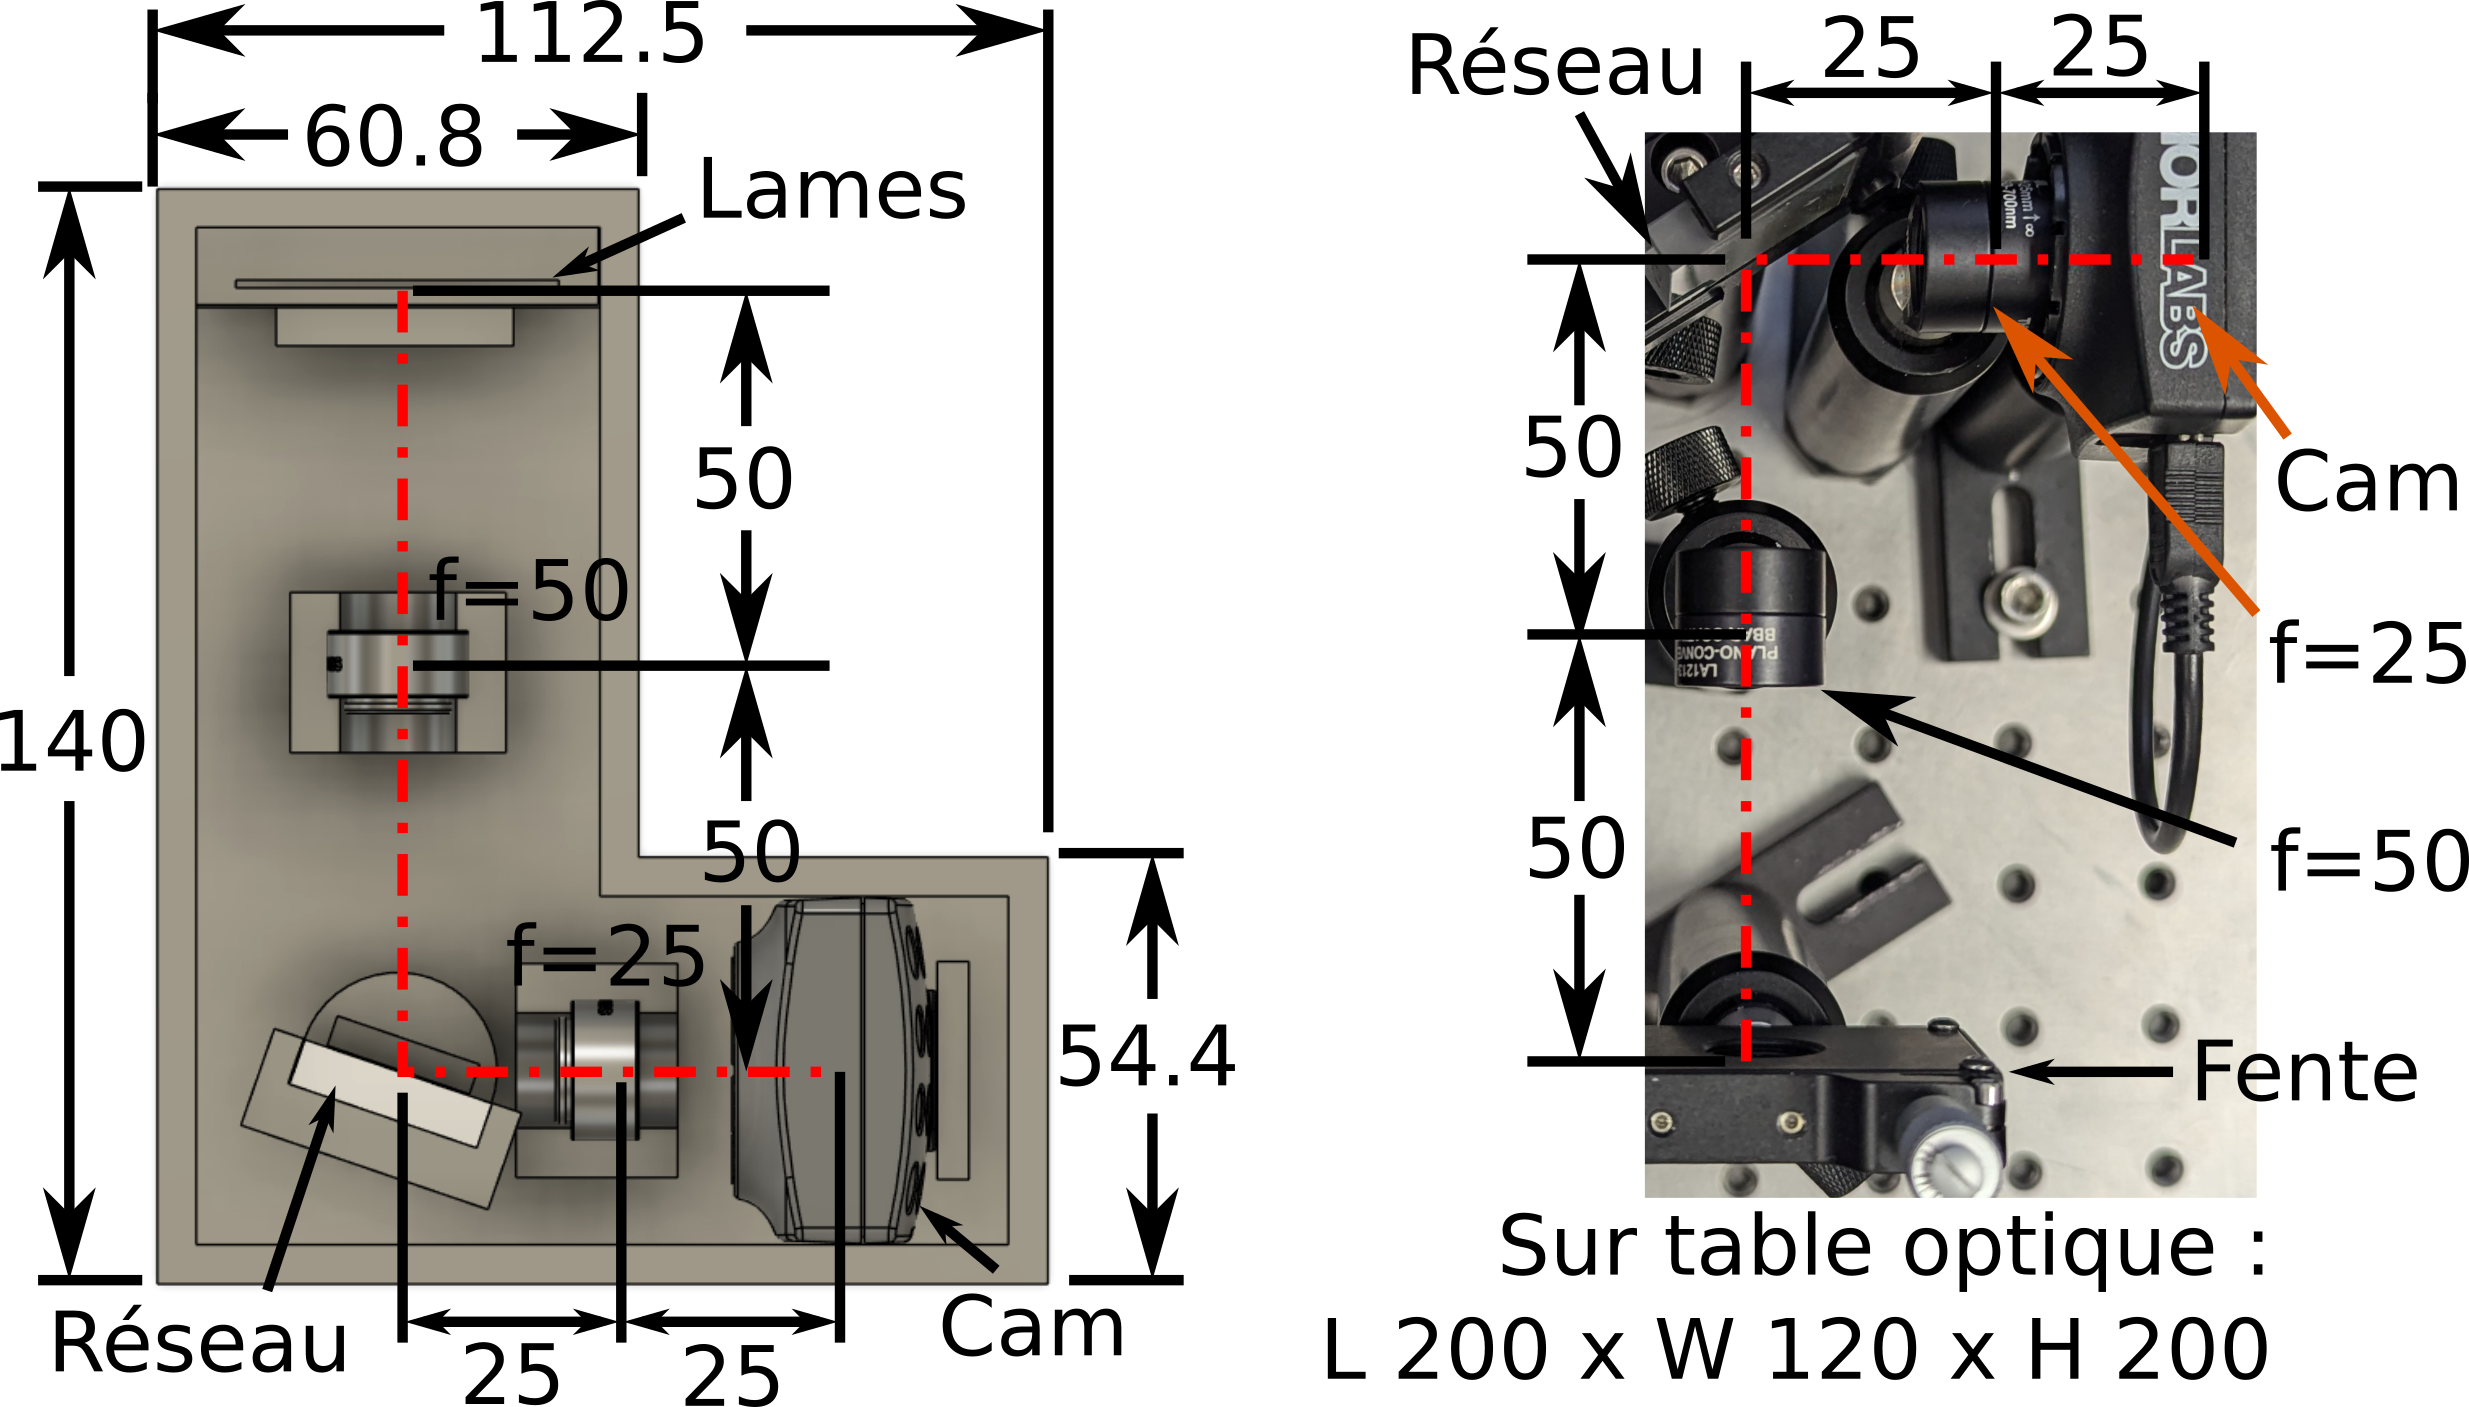
\includegraphics[scale=1.75]{schema_spectros.png}
  \caption{Schémas des spectromètres. Toutes les dimensions sont en millimètres. À gauche : spectromètre fait par impression 3D sans son couvercle. À droite : spectromètre sur table optique.}
  \label{schema_spectros}
\end{figure}

\begin{table}[H]
  \centering
  \caption{Tableau des spécifications}
  \begin{tabular}{|p{2.5cm}|p{2cm}|p{3cm}|p{1.5cm}|p{6.5cm}|}
  \hline
      Spectromètre & Résolution (nm) & Dimensions (mm) & Coût  \$CAD & Composantes \\ \hline\hline
      Table optique & ?? & L 200 $\times$ W 120 $\times$ H 200 & \$1,852.72 & \vspace{-20pt} {\small\parbox{7cm}{\setlength{\columnsep}{0pt} 
      \begin{multicols}{2}\begin{itemize}[label=$\triangleright$, topsep=0pt, itemsep=0pt]
            \item LA-1560-A-ML
            \item LA-1213-A-ML
            \item NE506A
            \item GR25-0605
            \item DCC1545M-GL
            \item VA100
            \item KM100S 
            \item SMR05 
            \item TR3-P5
            \item BA1
            \item BA1S
            \item PH6 
            \item PH4
            \item VC1 
        \end{itemize}
      \end{multicols} }} \\ \hline
      Impression 3D & ?? & L 140 $\times$ W 112.5 $\times$ H 80 & \$877.28 &  \vspace{-20pt} {\small\parbox{6.7cm}{\setlength{\columnsep}{-15pt} 
      \begin{multicols}{2}\begin{itemize}[label=$\triangleright$, topsep=0pt, itemsep=0pt]
            \item LA-1560-A-ML
            \item LA-1213-A-ML
            \item GR25-0605
            \item DCC1545M-GL
            \item Lames de rasoir
        \end{itemize}
    \end{multicols} } } \\ \hline
  \end{tabular}
  \label{specs}
\end{table}

\section{Rapports de tests}

L'objectif primaire de la construction de deux spectromètres séparés est de permettre la 
comparaison des coûts et de la performance des deux dispositifs. Cette section présente
donc les tests qui ont été effectués pour caractériser les dispositifs, et présente les 
conclusions quant à la performance des dispositifs.

\subsection{Conversion en longueurs d'onde et incertitude}

Pour caractériser la résolution, plusieurs étapes intermédiaires sont nécessaires. La procédure décrite ci-dessous est la même 
pour la table optique et pour le spectromètre imprimé en 3D. 
Les images obtenues à l'aide de la caméra et du logiciel Thorcam sont sous forme d'un fichier .tif.
Elles sont donc ouvertes sur python pour pouvoir traiter l'image sous forme de données brutes. Les fichiers tif 
contiennent des valeurs d'intensité entre 0 et 255 pour chaque pixel de la caméra. Il est important de mentionner
que lorsque la valeur excède 255, l'intensité est dite saturée, dans ce cas de figure le scripte python s'arrête et 
avertit l'utilisateur de la situation. Ces cas sont évités car l'information réelle sur le spectre est perdue.

Une fonction python est créée de façon à générer une courbe d'intensité en fonction de la position horizontale 
en pixel de la caméra. Pour ce faire, une sélection préalable est faite en choisissant uniquement les lignes 
contenant plus que 50 \% de l'intensité maximum, cette procédure permet de ne pas sélection les endroits de la caméra 
ou l'intensité est complètement nulle sur toute la longueur. Une fois cette opération achevée, la moyenne des intensités sur chaque
colonne est effectuée, ce qui retourne donc une valeur d'intensité pour chaque position de pixel horizontal. Cette étape est exécutée pour 
un laser bleu et un laser rouge.

Il est nécessaire de convertir l'échelle, initialement en pixel, en nanomètre.
Pour ce faire la formule suivante a été utilisée: 
\begin{align}
  \lambda =\frac{\lambda _{rouge}-\lambda _{bleu}}{x_{rouge}-x_{bleu}}(x-x_{bleu})-\lambda _{bleu}
\end{align}
Dans cette équation $\lambda $ représente la position horizontale avec une valeur en nm. Dans la même idée, 
$\lambda _{rouge}$ et $\lambda _{bleu}$ représentent la valeur en nm des pics d'intensité rouge et bleu. 
Pour sa part, x tout comme $x_{rouge}$ et $x_{bleu}$ représente une position sur une échelle en pixel.
Avec cette formule il est possible de générer un graphique, comme à la figure 2, de l'intensité d'un faisceau en fonction 
de sa longueur d'onde. 

Un aspect important à étudier qui n'est pas directement en lien avec la résolution est d'évaluer l'incertitude sur 
la position de nos pics d'intensité. Pour calculer cette incertitude, on utilise la formule suivante: 
\begin{align}
  \Delta \lambda =\sqrt{A^{2}+B^{2}+C^{2}}+\Delta \lambda _{bleu}
\end{align}
avec 
\begin{align}
  A=\frac{x-x_{bleu}}{x_{rouge}-x_{bleu}}\cdot \Delta\left ( \lambda _{rouge}-\lambda _{bleu} \right )
\end{align}
\begin{align}
  B=\frac{-(\lambda _{rouge}-\lambda _{bleu})\cdot (x-x_{bleu})}{(x_{rouge}-x_{bleu})^{2}} \cdot \Delta \left ( x_{rouge}-x_{bleu} \right )
\end{align}
\begin{align}
  C=\frac{(\lambda _{rouge}-\lambda _{bleu})}{(x_{rouge}-x_{bleu})}\cdot \Delta \lambda _{bleu}
\end{align}

Dans les équations ci-dessus, on définit $\Delta \lambda _{bleu}$ comme l'incertitude sur la la position (en nm)
du laser bleu. Dans le cas présent, la fiche technique du laser donne une incertitude de 5nm \cite{noauthor_compact_2024} . Pour la position en nm du laser bleu,
la valeur suivante sera donc utilisée: $ \lambda = 405\pm 5$ nm. On approxime que cette incertitude reste constante sur 
toutes les longueurs d'onde. Ainsi, il est obtenu que :
\begin{equation}
  \Delta\left ( \lambda _{rouge}-\lambda _{bleu} \right )=2\cdot \Delta \lambda _{bleu}. 
\end{equation}

Finalement le résultat suivant est donc obtenu : $\lambda _{rouge}-\lambda _{bleu}= (657-405)\pm 10$ nm.
Pour finir, on considère que l'incertitude sur la position de n'importe quelle position en pixel est la plus petite
division, soit 1 pixel. Le résultat suivant est donc obtenu: $\Delta \left ( x_{rouge}-x_{bleu} \right )=2$ pixels.

On remarque que l’incertitude sur la position varie de façon linéaire entre environ 5.5 et 15.5 nm, ce qui représente une
incertitude relative d'environ $1\%$ pour le bleu à 405 nm et d'environ $2\%$ pour le rouge à 657 nm. On remarque 
également que le terme dominant dans le calcul d'incertitude, 
c'est à dire qui contribue le plus à la valeur de l'incertitude, est le terme A. 
En fait, il s’agit plus précisément du terme $\Delta\left ( \lambda _{rouge}-\lambda _{bleu} \right )$ qui fait augmenter de beaucoup
la valeur de cette partie . On peut donc conclure qu'une façon efficace de réduire l'incertitude sur la position pour
les spectromètres est de réduire le plus possible l’incertitude sur la position du laser bleu. Puisque cette valeur d'incertitude
vient de la fiche technique du laser, on en déduit qu'il faudrait trouver un laser plus précis pour réduit l'incertitude 
globale de la position sur le spectromètre, ou qu'il faudrait étalonner le laser utilisé avec un autre appareil pour préciser
sa longueur d'onde centrale. 

%Partie 3: Largeur à mi-hauteur
% 1. Technique utilisée pour obtenir la largeur (maximum, positions à la moitié du max, un peu overshoot au cas où)
% 2. Comparaison entre les 3 spectromètres.

\subsection{Caractérisation de la résolution}

La résolution est définie comme étant la plus petite distance entre les centres de deux
faisceaux qui permet de les distinguer. On considère que lorsque les deux faisceaux se 
chevauchent à la moitié de leur intensité maximale, il n'est plus possible de les distinguer.
La largeur à mi-hauteur $FWHM$ de chaque faisceau sur le capteur est donc considérée. Pour 
caractériser l'appareil, on suppose que les faisceaux d'intérêt ont la largeur à mi-hauteur
du plus faisceau le plus étroit testé. La résolution est alors donnée par l'équation \ref{res}.

\begin{equation}\label{res}
  \text{Résolution} = \frac{1}{2}(FWHM_1)+\frac{1}{2}(FWHM_2)=\frac{2}{2}FWHM=FWHM
\end{equation}

Pour des faisceaux plus larges, ce ne serait pas la 
résolution du spectromètre qui limiterait la résolution obtenue, mais le profil des faisceaux
utilisés. Cela est cohérent, car il est préférable d'utiliser un appareil dans des cas où 
ce n'est pas sa résolution qui est limitante. 

La largeur à mi-hauteur est déterminée en trouvant les points ayant la moitié de l'intensité 
maximale. Ils sont toujours deux, de part et d'autre du centre, grâce au profil gaussien
des faisceaux laser, comme illustré à la figure \ref{FWHM_bleu}. Il suffit de prendre la 
différence entre les deux pour obtenir $FWHM$ et, donc, la résolution. 

\begin{figure}[h!]
  \centering
  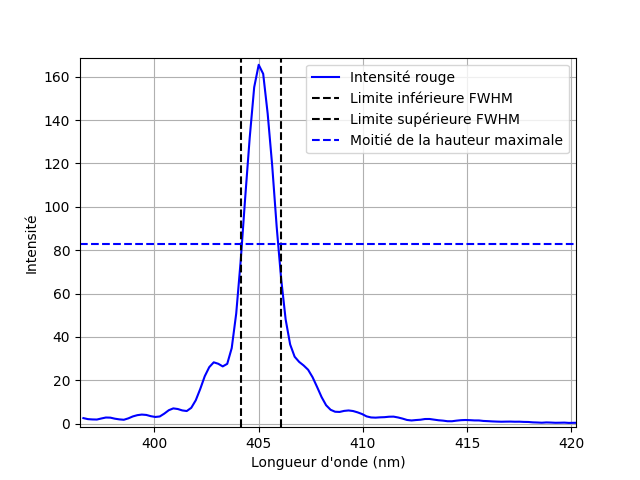
\includegraphics[width=0.8\linewidth]{FWHM_bleu_3D.png}
  \caption{Calcul de FWHM sur la courbe d'intensité obtenue pour le laser bleu avec le spectromètre imprimé en 3D. Zoom sur l'intervalle $[396, 420]$ nm}
  \label{FWHM_bleu}
\end{figure}

Dû à la nature discrète du spectre obtenu, il est courant que l'intensité à 
mi-hauteur ne corresponde pas directement à un point. Le point ayant l'intensité la plus proche
de la moitié de l'intensité maximale, tout en étant plus faible que celle-ci, est pris. De
cette façon, la largeur à mi-hauteur risque d'être légèrement surestimée, mais elle ne peut pas
être sous-estimée. L'incertitude sur cette mesure correspond à la plus petite divison de l'échelle en nm,
puisque, de chaque côté, on peut être légèrement décalé par rapport à la valeur définie précédement.

\subsection{Comparaison des deux spectromètres}

L'incertitude de la résolution est d'environ 0,4 nm et les résultats des résolutions 
obtenues sont présentés au tableau \ref{res_tab}.

\begin{table}[H]
  \centering
  \begin{tabular}{|c|c|c|}\hline
    Spectromètre & Résolution (nm) \\
    \hline
    Imprimé en 3D & 1,9 $\pm$ 0,4\\    \hline
    Sur table optique & 1,5 $\pm$ 0,4\\    \hline
  \end{tabular}
  \caption{Résolution pour les deux spectromètres testés}
  \label{res_tab}
\end{table}

La résolution obtenue pour le spectromètre sur table optique est de ($1,5 \pm 0,4$) nm, ce qui
est meilleur que celle obtenue pour le spectromètre imprimé en 3D, de ($1,9 \pm 0,4$) nm. Les difficultés d'alignement, qui sont plus importantes pour le spectromètre imprimé en 3D, ont
pesé dans la balance, notamment pour l'angle du réseau de diffraction et l'angle d'entrée du laser. 
En ajustant l'angle du réseau de diffraction, il arrive à de nombreuses reprises d'avoir 
le rouge ou le bleu sur la caméra, mais pas les deux.
Avec de multiples essais, l'alignement permettant d'avoir les deux simultanément est possible,
mais il peut s'accompagner d'aberrations provenant des lentilles, puisque les rayons extrêmes
se trouvent à passer très près du bord de celles-ci. Le système utilisé permet d'ajuster l'angle,
mais pas de le fixer, donc l'ajustement est à recommencer avant une série de prises de mesures si
l'appareil a été déplacé. 
L'angle d'entrée du laser importe puisqu'il détermine la position des rayons sur la caméra. Il doit
donc toujours être envoyé perpendiculairement à la fente pour des résultats répétables, ce qui est
plus facilement réalisable sur une table optique où le laser est maintenu à un endroit fixe par 
rapport au spectromètre.  

La fente affecte également la résolution, puisque sa largeur affecte directement la largeur du spectre
obtenu sur la caméra. Là encore, la table optique, avec un équipement plus couteux certes, permet un
contrôle de l'ouverture bien plus précis que les lames de rasoirs utilisées pour le spectromètre 3D.
L'espace entre celles-ci est plus large, ce qui affecte les résultats des tests. Il est également 
plus difficile d'assurer qu'elles forment une fentre rectangulaire, mais cet élément n'affecte pas 
la résolution de manière conséquente étant donné le traitement fait sur les données.
La table optique a pour sa part une limitation majeure; il y est plus difficile de s'assurer que les
lentilles sont positionnées au bon endroit, c'est-à-dire à une longueur focale de l'élément qui la 
précède et qui la suit. Cela pourrait avoir comme effet de rendre l'image plus floue, car les principes
utilisés ne sont valables que pour une configuration 4f, donc en ayant une configuration approximative,
il y a risque de rendre l'image approximative, donc de nuire à la résolution. 

Les tests des deux spectromètres avec un laser rouge sont présentés et comparés au résultat d'un 
spectromètre commercial. La largeur à mi-hauteur du laser rouge obtenue avec chaque spectromètre est 
présentée au tableau \ref{res_tab_rouge}. L'incertitude sur la résolution du spectromètre commercial 
est prise comme la plus petite graduation sur l'échelle des longueurs d'onde, soit 0,8 nm.

\begin{table}[H]
  \centering
  \begin{tabular}{|c|c|c|}\hline
    Spectromètre & Largeur à mi-hauteur (nm) \\
    \hline
    Imprimé en 3D & 8,0 $\pm$ 0,4\\    \hline
    Sur table optique & 2,3 $\pm$ 0,4\\    \hline
    Commercial & 12,1 $\pm$ 0,8\\    \hline
  \end{tabular}
  \caption{Résolution pour les deux spectromètres testés et le spectromètre commercial}
  \label{res_tab_rouge}
\end{table}

Aucun des deux spectromètres n'obtient la même largeur à mi-hauteur que le spectromètre commercial.
La largeur à mi-hauteur obtenue avec le spectromètre sur table optique, de $(2,3 \pm 0,4)$ nm, est 
beaucoup plus faible que celles obtenues avec le spectromètre imprimé en 3D, de $(8,0 \pm 0,4)$, nm 
ou avec le spectromètre commercial, de $(12,1 \pm 0,8)$ nm. Les deux spectromètres s'accordent sur 
le fait que le laser rouge a un profil plus large que le laser bleu.

Alors que pour le bleu, les spectromètres tombent d'accord, il n'y a pas de largeur à mi-hauteur
commune donnée par les trois spectromètres. Cela peut être dû à une combinaison des aberrations 
des lentilles, aux enjeux d'alignement, de positionnement des éléments optiques et de contrôle de
la fente. Le laser rouge ayant un profil plus large, il est plus sujet aux aberrations des lentilles
qui n'affectent pas le faisceau églement en fonction de la position (extrême au centrale) où elle
est traversée. Il est également plus sujet aux clippage à cause de sa largeur. Pour couronner le tout,
ce laser n'est pas aligné avec son boitier, donc il est probable qu'il n'entre pas correctement dans
le système optique. 

Sans avoir d'information sur le spectromètre commercial utilisé, la confiance est tout de même supérieure
pour le résultat obtenu avec ce spectomètre. Les spectromètres semblent donc sous-estimer la largeur deux
laser rouge testé, avec un effet moins prononcé pour le spectromètre imprimé en 3D que celui sur table optique.
Les spectres de diodes électroluminescentes testées sont toutefois cohérents, ce qui semblerait indiquer que 
cette aberration des systèmes est davantage un enjeu pour les longueurs d'onde extrêmes tirant sur le rouge,
plutôt que pour tout le spectre. 

% # Partie 4: Conclusion
% # 1. Comparaison entre les 2 spectros: Table optique meilleure
% # 2. Limitations de cette comparasion: Difficultés d'alignement ++pour le 3D spécifiquement (angle du réseau de diffraction),
% # angle du laser devrait être perpendiculaire à la fente: difficle à confirmer pendant les tests surtout pour 3D, de 
% # , aberration des lentilles,
% # qualité des photos photo obtenues, qualité de la fante fabriquée avec des lames de rasoirs (pas tellement droite, gros espace)
% positionnement des lentilles à leur focale
% # 3. Comparaison avec Datasheet du bleu et
% résultat du rouge (énoncer leur résultat et dire qu'est-ce qui est plus grand que quoi)
% # 4. Limitations de cette comparaison: qualité du laser (angle par rapport au boitier du laser lui-même)
% # Comparer les deux spectro (table et 3D) au spectro de Guillaume. 

% Donner l'incertitude relative


\subsection{Rapport détaillé des coûts}

Les méthodes de construction étant grandement différentes pour les deux spectromètres, une 
étude des coûts est faite afin de déterminer lequel des deux est le plus abordable. Pour ce
faire, une liste détaillée des pièces requises est faite, et le total des coûts est calculé en
dollars canadiens avant taxes. Sauf exception, tous les prix proviennent de Thorlabs \cite{noauthor_thorlabs_2024}. La table \ref{prix_table} présente les coûts des pièces pour
le système monté sur table optique :

\begin{table}[!ht]
    \centering
    \caption{Liste des pièces et coûts totaux pour le spectromètre sur table optique \cite{noauthor_thorlabs_2024}}
    \begin{tabular}{|l|l|c|r|r|}
    \hline
        ID pièce & Description & Qté & \$ CAD & Total ind. \\ \hline\hline
        LA-1560-A-ML & Lentille plano-convexe f=25 mm & 1 & \$72.25 & \$72.25 \\ \hline
        LA-1213-A-ML & Lentille plano-convexe f=50 mm & 1 & \$70.61 & \$70.61 \\ \hline
        NE506A & Filtre atténuateur de lumière & 2 & \$59.55 & \$119.10 \\ \hline
        GR25-0605 & Réseau de diffraction 600/mm & 1 & \$178.32 & \$178.32 \\ \hline
        DCC1545M-GL & Caméra USB & 1 & \$539.21 & \$539.21 \\ \hline
        VA100 & Fente ajustable & 1 & \$417.74 & \$417.74 \\ \hline
        KM100S & Montage à réseau de diffraction & 1 & \$130.45 & \$130.45 \\ \hline
        SMR05 & Trou taraudé pour lentilles & 2 & \$28.68 & \$57.35 \\ \hline
        TR3-P5, & 5 tiges pour optiques & 1 & \$38.50 & \$38.50 \\ \hline
        BA1 & Pied de montage optique & 2 & \$8.42 & \$16.85 \\ \hline
        BA1S & Pied de montage optique & 4 & \$7.83 & \$31.30 \\ \hline
        PH6 & Base pour tiges d'optique & 5 & \$20.43 & \$102.17 \\ \hline
        PH4 & Base pour tiges d'optique & 1 & \$14.83 & \$14.83 \\ \hline
        VC1 & Pince en V & 1 & \$64.04 & \$64.04 \\ \hline\hline
        ~ & ~ & ~ & Total : & \$1,852.72 \\ \hline
    \end{tabular}
    \label{prix_table}
\end{table}

Quelques points sont à relever pour cette table. La caméra utilisée est maintenant indisponible
à l'achat sur le site de Thorlabs. Le prix affiché est donc le prix de cette pièce avant
qu'elle soit enlevée du site en 2021 \cite{noauthor_thorlabs_2021}. Aussi, deux éléments importants
ont été omis de cette liste. La quincaillerie, soit les vis, les écrous et les 
rondelles, n'ont pas été comptées car ces derniers sont fréquemment disponibles en vrac dans
des ateliers, ou ils s'achètent en ensemble à moindre coût. La table pour fixer les éléments 
optiques n'a pas été comptée non plus car elle ne servait pas que pour le spectromètre 
construit. Sa taille, donc son prix est donc beaucoup trop grand par rapport au besoin du projet. L'appareil
construit fonctionnerait sur la table B1212F, mesurant 12 x 12 po. Avec un coût de 966.85\$,
le total serait amené à 2819.57\$. L'achat de cette table pourrait toutefois ne pas être 
justifiable pour un laboratoire étant donné sa taille restreinte, donc des options plus grandes
seraient à considérer.

% source A : https://www.thorlabs.com/thorProduct.cfm?partNumber=DCC1545M

La table \ref{prix_3D} montre le calcul des coûts pour le modèle fait par l'impression 3D :

\begin{table}[!ht]
    \centering
    \caption{Liste des pièces et coûts totaux pour le spectromètre avec impression 3D \cite{noauthor_thorlabs_2024} \cite{noauthor_razor_2024}}
    \begin{tabular}{|l|l|c|r|r|}
    \hline
        ID pièce & Description & Qté & \$ CAD & Total ind. \\ \hline\hline
        LA-1560-A-ML & Lentille plano-convexe f=25 mm & 1 & \$72.25 & \$72.25 \\ \hline
        LA-1213-A-ML & Lentille plano-convexe f=50 mm & 1 & \$70.61 & \$70.61 \\ \hline
        GR25-0605 & Réseau de diffraction 600/mm & 1 & \$178.32 & \$178.32 \\ \hline
        DCC1545M-GL & Caméra USB & 1 & \$539.21 & \$539.21 \\ \hline
        - & Impression 3D & 1 & \$6.94 & \$6.94 \\ \hline
        - & Ensemble de lames de rasoir & 1 & \$9.95 & \$9.95 \\ \hline\hline
        ~ & ~ & ~ & Total : & \$877.28 \\ \hline
    \end{tabular}
    \label{prix_3D}
\end{table}

Un élément a aussi été exclu de cette liste, soit l'imprimante 3D utilisée pour l'impression.
Celle utilisée, soit la Original Prusa i3 MK3S+, est disponible pour 899\$ US, ou 1245.21\$ CAD \cite{prusa_imprimante_2024} .
Si considéré, ce prix augmente grandement les coûts associé à ce modèle de spectromètre, étant
plus dispendieux que le total calculé. Toutefois, ce type d'imprimante est facilement accessible
gratuitement en faisant affaire avec certains ateliers. Aussi, pour de faibles quantités de
pièces, il est possible de commander des impressions en ligne pour beaucoup moins cher que
l'imprimante. C'est donc pourquoi son prix a été omis.

Il est donc facile de conclure que l'impression 3D est beaucoup plus avantageux économiquement.
Le prix de l'impression sous 10\$ est une très grande économie lorsque comparé aux nombreuses
pièces servant au montage sur table optique qui ont fortement contribués au coût élevé du
modèle qui les requiert. L'économie de 975.44\$ en allant avec le modèle imprimé est
considérable, et étant donné sa performance respectable, c'est le modèle à préconiser.



% \clearpage
% \printbibliography
\bibliographystyle{unsrtnat}
\bibliography{spectro.bib}

\end{document}
